\documentclass[11pt,border=0mm,tikz]{standalone}
\usepackage{csquotes}
\usepackage[backend=biber,style=numeric,sorting=none]{biblatex}

\providecommand{\FigScale}{1}

\usepackage{siunitx}
\usepackage{tikz}
\usetikzlibrary{decorations.pathmorphing,patterns}
\usetikzlibrary{shapes.geometric, arrows.meta}
\usetikzlibrary{positioning}

\usepackage{amsmath}
\usepackage{upgreek}
\usepackage{svg}

\usetikzlibrary{3d}
\usetikzlibrary{calc}

\tikzset{
box/.style={
	rectangle,
	rounded corners=4pt,
	minimum width=3cm,
	minimum height=1cm,
	text centered,
    align=center,
	draw=black!70,
	line width=0.95pt,
	fill=gray!5,
	inner sep=4pt
},
circlebox/.style={
	circle,
	minimum size=1.5cm,
	text centered,
	draw=black!70,
	line width=0.95pt,
	fill=gray!5,
	inner sep=1pt
},
arrow/.style={
	thick,
	->,
	>=Stealth,
	draw=black!70,
	line width=1pt,
	line cap=round,
	line join=round,
	shorten <=1pt,
	shorten >=1pt
}
}

\begin{document}

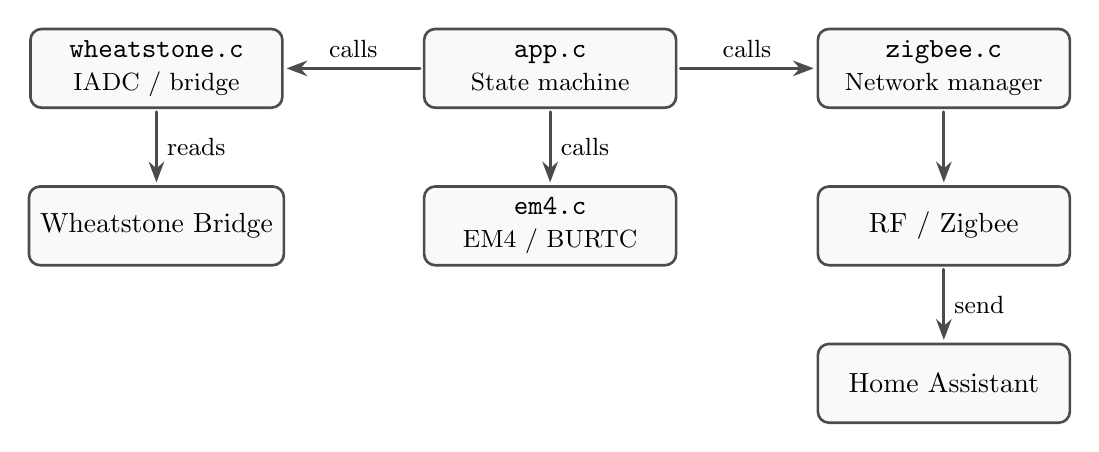
\begin{tikzpicture}[scale=\FigScale, node distance=2cm]

\node (app)  [box, minimum width=3.2cm] {\texttt{app.c}\\{\small State machine}};
\node (zig)  [box, right of=app, xshift=3cm, minimum width=3.2cm] {\texttt{zigbee.c}\\{\small Network manager}};
\node (whs)  [box, left of=app, xshift=-3cm, minimum width=3.2cm] {\texttt{wheatstone.c}\\{\small IADC / bridge}};
\node (em4)  [box, below of=app, minimum width=3.2cm] {\texttt{em4.c}\\{\small EM4 / BURTC}};

\node (bridge) [box, below of=whs, minimum width=3.2cm] {Wheatstone Bridge};
\node (radio)  [box, below of=zig, minimum width=3.2cm] {RF / Zigbee};
\node (HA)     [box, below of=radio, minimum width=3.2cm] {Home Assistant};

\draw [arrow] (app.east) -- node[midway, above, font=\small] {calls} (zig.west);
\draw [arrow] (app.south) -- node[midway, right, font=\small] {calls} (em4.north);
\draw [arrow] (app.west) -- node[midway, above, font=\small] {calls} (whs.east);
\draw [arrow] (whs.south) -- node[midway, right, font=\small] {reads} (bridge.north);
\draw [arrow] (zig.south) -- node[midway, right, font=\small] {} (radio.north);
\draw [arrow] (radio.south) -- node[midway, right, font=\small] {send} (HA.north);

\end{tikzpicture}

\end{document}